\chapter{Neural Recommender Systems for Conversational Recommendation Systems}
\chaptermark{Neural Recommender system Design}
\label{ch:recommender} % Label for main chapter

\section{Introduction}

Neural recommender systems provide a flexible approach to adapt architectures according to the specific demands of a given system. Particularly, when dealing with dialogue-based scenarios, such systems require the accumulation of user profile information over multiple conversational turns. In this context, sequence models, such as architectures based on Long Short-Term Memory (LSTM), and attention mechanisms are particularly suitable. These models excel at capturing the complex dynamics of user interactions, thereby enabling more nuanced and effective recommendations within dialogue-driven recommendation systems. 

\begin{itemize}
    \item The user's representation should be based on their preference history, which consists of a set of item-rating pairs obtained during the dialogue, not user ID. Cold start scenario is assumed at the beginning of the dialogue, which means that user ID is not available when pre-training the recommender module.
    \item Recommendation quality should improve consistently as new item-rating inputs are added to the model, as difference in the model recommendation quality will be used as a reward in the policy component.
\end{itemize}

In this chapter propose a novel architecture for a recommender module that is specifically designed to meet the criteria listed above, paving the way for improved dialogue-driven recommendation systems.


\section{Methodology}
\label{ch:method} % Label for method chapter

\subsection{Datasets}
The first dataset is generated artificially with the goal of making the development, debugging and evaluation of the algorithm as transparent as possible. The dataset consists of Boolean values that represent movie ratings assigned by $n$ users to $k$ movies. The matrix is complete, meaning that all users have ratings for all movies. Perfect collinearity is introduced in this dataset in order to evaluate the ability of the algorithm to select items that maximise information gain. Specifically, the movie set consists of $k/2$ independent clusters, containing two perfectly correlated movies each. Thus, if the conversational agent observes the rating of one of the movies in a cluster, asking about the second movie would not allow it to further improve the accuracy of its internal representation of the user's tastes.

The second dataset follows a similar format, however, it is generated based on real user ratings. In order to emulate a realistic and human-like information exchange between the \textit{ABot} and the \textit{QBot}, it has been enriched with movie attributes. Firstly, \textit{MovieLens} dataset \citep{harper2015movielens} was used as a source of collaborative data. The number of distinct movies was limited to the 100 most frequently rated titles, and the number of user was limited to those who has at least a quarter of ratings available (37,139 users in total). Secondly, the dataset was enriched with several movie attribute categories: genre, cast \& crew and plot keywords. The movie metadata was obtained from \textit{Kaggle.com} and is based on \textit{TMDB} and \textit{GroupLens} datasets.

Cast \& crew feature space was constrained to contain only the most well-known actors (top 50) and movie directors (top 50) in order to reduce the dimensionality of the input feature matrix. Cast \& crew popularity $p$ was not directly available in the dataset and was approximated by dividing movie vote count $v$ (as a proxy for movie popularity) by cast member's order of appearance in the credits $k$ (as a proxy for their importance to the success of the movie) and summing over the movies $M$ that the cast member appeared in:

\begin{equation} 
\label{eq:cast_popularity}
p_{i}=\sum_{j=1}^{n}\frac{v_{j}}{(k_{ji}+1)}
\end{equation}

It has been shown that in natural unscripted human conversations, users don’t just rely on easily available movie metadata (e.g., year, genre); rather, they often use less well defined properties such as story, plot, characters, acting and attributes like violence \citep{radlinski2019coached}. To address this gap, a set of common keywords mined from movie plots has been added to the dataset.


\subsection{Algorithms} %% call specific name - based on algorithm

I propose a novel architecture for a recommender module that utilizes an item-to-item approach in order to predict movie ratings. This approach enables the module to make predictions for new users whose user ID was not previously observed and included in the model training data. A Long Short-Term Memory (LSTM) network with attention mechanism is used to predict the full vector of user’s ratings $V_u$ from a shuffled partially observed history of ratings $s_t$. Attention mechanism allows the network to learn the relationships between inputs and outputs directly based on embedded indexes of movies and independently of the order of inputs, which can be arbitrary. 

The \textit{recommendation} network $\phi$ receives a movie index $a_t$ and a rating $v_a$ at each timestep $t$. The rating $v_a$ is one-hot encoded and can belong to one of the three categories that capture a combination of implicit and explicit ratings: (a) liked, (b) disliked, (c) not rated. It embeds the index (embeddings are learned in the process of optimisation), concatenates the embedding with the rating and passes the resulting vector to an LSTM unit, which learns an encoded representation of a user’s history. At each timestep, this representation is decoded by passing the LSTM hidden state through two dense hidden layers. The encoded state is connected to decoder outputs with the attention mechanism. Outputs of the decoder and the attention layer are concatenated and passed through the final dense layer with a sigmoid nonlinearity function. A set of movie ratings $V_u$ drawn from a user’s history serve as model ground truth values. Movie IDs that have no available ratings $v_t$ for a given user (in MovieLens dataset) are masked during the calculation of cross-entropy function. 

The network is trained through backpropagation using the Adam optimisation algorithm to minimise cross-entropy loss $minL(\Theta_{rec})$, where

\begin{equation} 
\label{eq:recommender_loss}
L(\Theta_{rec})=-V\log(\phi(s_t))-(1-V)log(1-\phi(s_t))
\end{equation}

where $\phi(s_t)$ is the output of the \textit{recommendation} neural network given the state $s_t$. 

The \textit{recommendation} network is trained independently on the full user history. Its hidden layers serve as a bottleneck that forces the network to learn to predict ratings of unobserved movies based on correlated observed movies. Therefore, a new observation of a movie-rating pair reduces the loss most when it is uncorrelated with previous observations and information gain is maximised. The between-timestep difference in loss of the \textit{recommendation} network will serve as a reward observed by the \textit{policy} network $\pi$.


\section{Results}

Good performance of the recommendation network is a prerequisite of successful training of the Questioner’s policy network. The recommendation network is trained to predict the full set of ratings based on the partial set, therefore, at the last timestep of the recurrent network it is expected to have approximately zero cross-entropy loss, which would confirm that the network has learned to correctly map inputs to outputs based on movie indexes and that intermediate bottleneck layers do not result in information loss. Indeed, the model trained on MovieLens dataset achieves loss of 0.07 as can be seen in Figure~\ref{fig:rec_all}. 

\begin{figure}[ht]
    \centering
    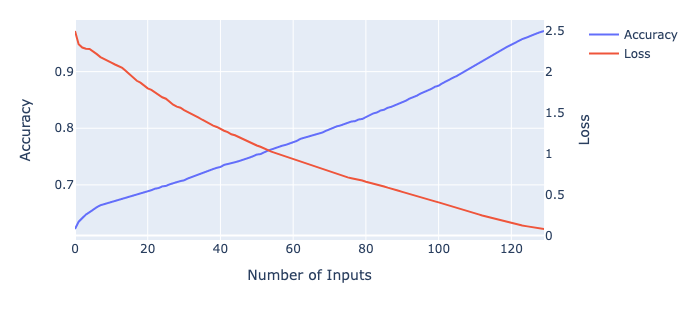
\includegraphics[scale=0.5]{figures/rec_all.png}
    \caption{Recommendation network accuracy and loss improvement by number of inputs drawn from MovieLens dataset}
    \label{fig:rec_all}
\end{figure}

Furthermore, we would expect the loss to decrease as a function of the number of inputs, as more and more of a user’s history is revealed through conversation. Looking at the curve shown in Figure~\ref{fig:rec_all}, we can see that at each timestep entropy is reduced, however, information gain gradually slows down as a function of number of timesteps, which suggests that the model can successfully learn to extrapolate from the incomplete available data.

\clearpage
This observation is confirmed by the fact that the model can successfully predict ratings of movies that have not been passed as model inputs. Figure~\ref{fig:rec_holdout} shows that prediction accuracy consistently improves with the increase in the number of inputs where sets of input and output movies do not overlap improving average prediction accuracy from the baseline 0.6 to 0.8.

\begin{figure}[ht]
    \centering
    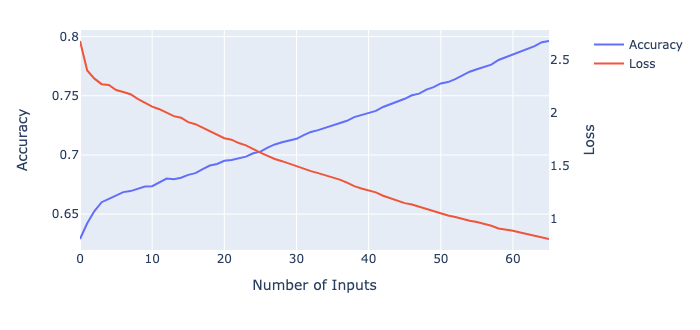
\includegraphics[scale=0.5]{figures/rec_holdout.png}
    \caption{Recommendation network accuracy and loss improvement on a MovieLens holdout set of movies by number of inputs}
    \label{fig:rec_holdout}
\end{figure}

To sense check the model, we can observe how the recommendation model behaves in the scenario when some movies are perfectly correlated. We have introduced perfect collinearity in the synthetic dataset. The dataset contains five clusters, each consisting of two perfectly correlated rating vectors. Figure~\ref{fig:rec_redundant_info} compares model loss in three scenarios: (1) when the full user’s history is observed, (2) when half of the movies are observed, each drawn from a separate cluster, and (3) when half of the movies are observed, but the movies are drawn at random. We can see that the second scenario results in near perfect loss (0.02), which is similar to the first scenario, which suggests that the model has successfully learned to recreate the full information from a partially observed history. In contrast to that, the third scenario, where information is incomplete, results in high loss, as expected.

\begin{figure}[ht]
    \centering
    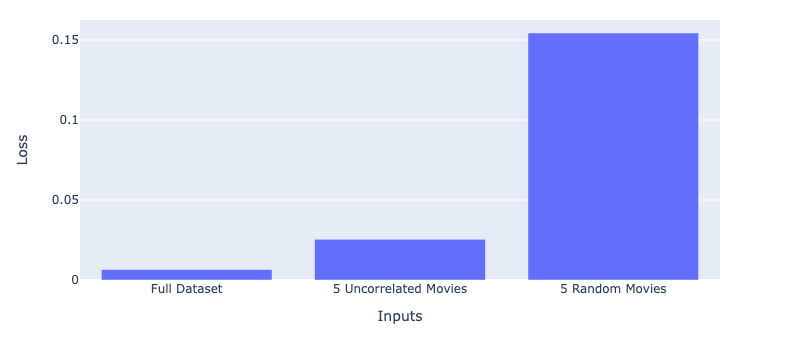
\includegraphics[scale=0.5]{figures/rec_redundant_info.png}
    \caption{Recommendation network loss obtained on the synthetic dataset as a function of entropy in input data}
    \label{fig:rec_redundant_info}
\end{figure}

\clearpage
\begin{figure}[ht]
    \centering
    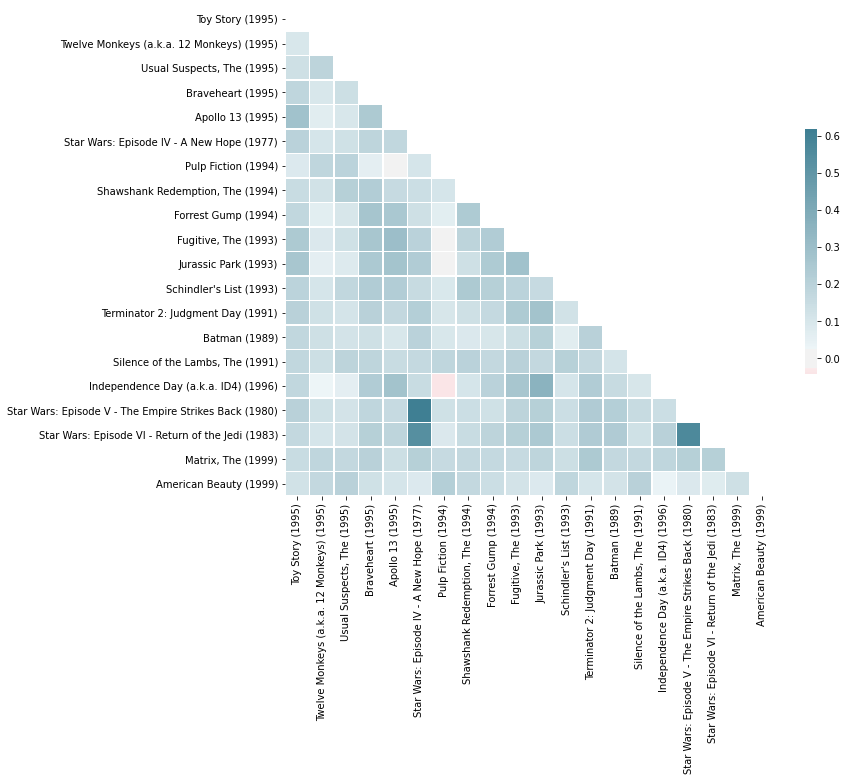
\includegraphics[scale=0.35]{figures/movielens_corr.png}
    \caption{Pairwise Pearson’s correlation coefficients between pairs of rating vectors corresponding to movies drawn from the MovieLens dataset}
    \label{fig:movielens_corr}
\end{figure}

The natural dataset drawn from MovieLens does not have perfectly correlated movies, however, it does have a distinct rating cluster formed by different episodes of ‘Star Wars’ (see Figure~\ref{fig:movielens_corr}). Figure~\ref{fig:sw_corr} shows that the loss is considerably lower when predicting the rating given to Episode IV if either Episode V or Episode VI are observed, compared to loss of the rating prediction based on other movies in the dataset.

\begin{figure}[ht]
    \centering
    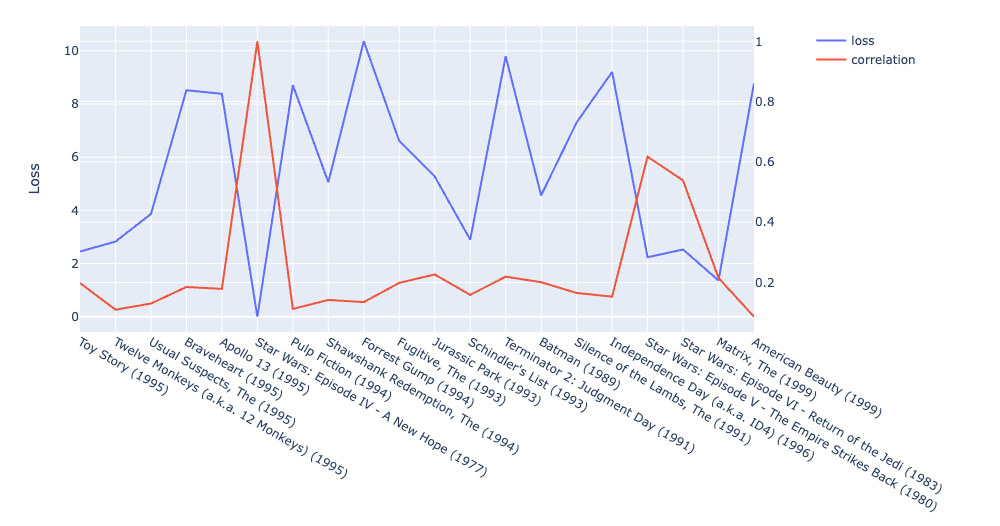
\includegraphics[scale=0.3]{figures/sw_corr.png}
    \caption{Pairwise Pearson’s correlation coefficients between pairs of rating vectors corresponding to movies drawn from the MovieLens dataset}
    \label{fig:sw_corr}
\end{figure}

\clearpage
Previous research has shown that movie attributes play a significant role in natural conversations surrounding films. To enable Questioner and Answerer bots to use this in their interactions, the dataset has been enriched with attribute ratings, including actor, director and genre which were derived from movie ratings. The graph below illustrates the model's performance in predicting movie ratings solely based on attribute ratings. As demonstrated, the model has effectively learned the relationships between attributes and items, and leverages this information to make predictions, albeit with slightly lower accuracy than item-to-item predictions.

\begin{figure}[ht]
    \centering
    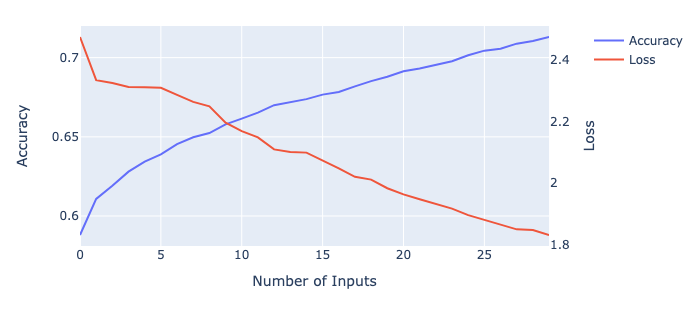
\includegraphics[scale=0.5]{figures/rec_attributes.png}
    \caption{Recommendation network accuracy and loss improvement on movies by number of attribute inputs}
    \label{fig:rec_attributes}
\end{figure}

In order to verify the meaningfulness of model mappings between attributes and individual movies, we have manipulated the ratings of attributes and measured the changes in predictions, which allowed to identify the most affected items. As an illustration, we have examined the effect of attribute ratings on movie recommendations, where the only known attribute is ``Russell Crowe" and observed that positive ratings of this attribute improve the predictions for related movies, such as ``A Beautiful Mind," ``Gladiator," and ``L.A. Confidential," which aligns with the expected outcomes (see Table~\ref{tab:crowe}).

\begin{table}[h!]
    \centering
    \caption{Top 10 improved movie ratings when attribute "Russell Crowe" was manipulated}
    \label{tab:crowe}
    \begin{tabular}{llr}    
        \toprule
        \cmidrule(r){1-2}
        Title & Rating Difference \\
        \midrule
        ``The Silence of the Lambs" & +1.00\\
        ``Apollo 13" & +0.94\\
        ``The Princess Bride" & +0.94\\
        ``The Godfather" & +0.92\\
        ``The Mask" & +0.92\\
        ``A Beautiful Mind" & +0.91\\
        ``Gladiator" & +0.89\\
        ``Jurassic Park" & +0.88\\
        ``Clear and Present Danger" & +0.83\\
        ``L.A. Confidential" & +0.82\\
        \bottomrule
    \end{tabular}
\end{table}